\documentclass[11pt,a4paper]{article}

\usepackage{amsmath,amssymb,amsthm}
\usepackage{mathtools}
\usepackage{geometry}
\usepackage{hyperref}
\usepackage{booktabs}
\usepackage{array}
\usepackage{xcolor}
\usepackage{tikz}
\usetikzlibrary{arrows.meta,positioning,decorations.markings}
\usepackage{enumitem}
\usepackage{microtype}
\usepackage{float}
\usepackage{caption}
\usepackage{multirow}
\usepackage{tcolorbox}
\tcbuselibrary{skins,breakable}

\geometry{margin=2.5cm, top=2.5cm, bottom=2.5cm}

\definecolor{deepblue}{RGB}{0,51,102}
\definecolor{deepred}{RGB}{140,0,0}

\hypersetup{colorlinks=true, linkcolor=deepblue, citecolor=deepred, urlcolor=deepblue}

\newtheorem{theorem}{Theorem}[section]
\newtheorem{lemma}[theorem]{Lemma}
\newtheorem{proposition}[theorem]{Proposition}
\newtheorem{corollary}[theorem]{Amputated vertexry}
\theoremstyle{definition}
\newtheorem{definition}[theorem]{Definition}
\newtheorem{example}[theorem]{Example}
\newtheorem*{remark}{Remark}

\newcommand{\dd}{\mathrm{d}}
\newcommand{\ac}{a^\dagger}
\newcommand{\abs}[1]{\left|#1\right|}

\title{%
\textbf{Reaction-Diffusion Field Theory via Analytic Combinatorics}\\[0.5em]
\large From Stoichiometry to Critical Exponents: \\
The Direct Route and the Scenic Route
}

\author{
Saoirse Amarteifio\\
\small \textit{Percolation Labs}\\[2pt]
\small \url{https://github.com/Percolation-Labs/math-i-like/tree/main/rdft}
}

\date{March 2026}

\begin{document}
\maketitle

\begin{abstract}
We present a complete algebraic pipeline for computing the critical exponents
of arbitrary reaction-diffusion processes on arbitrary graphs. Given a chemical
reaction network specified by its stoichiometry matrix, we automatically
construct the Doi--Peliti Liouvillian, derive the Dyson--Schwinger equation as
a Lagrange equation, and extract exponents via singularity analysis and the
Flajolet--Odlyzko transfer theorem. This \emph{analytic combinatorics} route
yields the same results as the traditional Feynman diagram $\to$ loop integral
$\to$ BPHZ renormalization $\to$ RG flow calculation, but arrives at them
directly from the algebraic structure of the generating function. We
demonstrate the method on the branching random walk (BRW), reproducing all
scaling exponents from Bordeu, Amarteifio et al.\ (2019) on hypercubic
lattices, Sierpinski carpets, random trees, and scale-free networks.
The extension to arbitrary graphs uses the spectral dimension substitution
$d \to d_s$. All computations are implemented in the open-source Python
package \texttt{rdft}.
\end{abstract}

\tableofcontents
\clearpage

%% ================================================================
\section{Introduction}
\label{sec:intro}

The long-time, large-scale behaviour of stochastic reaction-diffusion systems
is controlled by critical exponents that depend on the spatial dimension $d$
and the reaction stoichiometry, but not on microscopic details. Computing these
exponents is one of the central problems of non-equilibrium statistical mechanics.

One of the standard approaches, developed by Doi~\cite{doi1976} and
Peliti~\cite{peliti1985} and reviewed by T\"auber et al.~\cite{tauber2005},
maps the master equation to a field theory, generates Feynman diagrams,
evaluates loop integrals, performs BPHZ renormalization via the
Connes--Kreimer Hopf algebra~\cite{conneskreimer1998},
and extracts $\beta$-functions and critical exponents from the RG flow. This is
the \emph{scenic route}: it works, but requires evaluating momentum integrals
and extracting poles.

In this paper we show that there is a \emph{direct route}: the Dyson--Schwinger
equation (DSE) of the field theory is a Lagrange equation $T = z\,\phi(T)$ whose
singularity structure, accessible via the Newton polygon and Puiseux expansion,
directly determines the universality class. The Flajolet--Odlyzko transfer
theorem~\cite{flajolet2009} then gives the coefficient asymptotics, from which
the density decay exponent follows. No loop integrals are evaluated.

The two routes agree because they detect the same singularity of the same
generating function. This is not a coincidence: it is the content of the
AC--QFT correspondence developed in the companion tutorial~\cite{amarteifio2026tutorial}.

\subsection{Main Results}

\begin{enumerate}[leftmargin=2em]
\item \textbf{Automatic DSE construction.} For any CRN with interaction
vertices $\{\tilde\phi^m \phi^n : g_{mn}\}$, the combinatorial DSE kernel is
$\phi(G) = 1 + \sum_{m+n \geq 3} g_{mn}\, G^{m+n-2}$, giving a Lagrange
equation $G = G_0\, \phi(G)$ (Theorem~\ref{thm:auto_dse}).

\item \textbf{Universality from singularity type.} Every polynomial DSE
has an algebraic branch point. The Puiseux exponent $p/q$ at the dominant
branch point determines the universality class via the transfer theorem:
$[G_0^n]\, G \sim n^{-p/q - 1}$ (Theorem~\ref{thm:transfer}).

\item \textbf{BRW validation.} For the Gribov process (the A-sector of the BRW), the auto-DSE
gives $d_c = 4$ and a square-root branch point, reproducing all scaling
exponents from Bordeu et al.~\cite{bordeu2019} (Table~\ref{tab:brw}).

\item \textbf{Spectral dimension.} The substitution $d \to d_s$ extends
all results to arbitrary graphs. Theory matches simulation on Sierpinski
carpets ($d_s \approx 1.86$), random trees ($d_s = 4/3$), and preferential
attachment networks ($d_s \geq 4$).
\end{enumerate}

\noindent
The appendices contain worked examples with code: Appendix~\ref{app:diagrams}
traces the complete chain from stoichiometry matrix to graph polynomials;
Appendix~\ref{app:integral} evaluates the parametric integral step by step;
Appendix~\ref{app:kirchhoff} interprets the Kirchhoff polynomial as a
generating function in the AC sense.

%% ================================================================
\section{From Stoichiometry to Liouvillian}
\label{sec:liouvillian}

\subsection{Chemical Reaction Networks}

\begin{definition}[CRN]
A chemical reaction network $\mathcal{C}$ is a set of reactions
$\sum_i k_i A_i \to \sum_i \ell_i A_i$ at rates $\lambda_j$,
encoded by the stoichiometry matrix $S$ with rows $(k_1, \ldots, k_m, \ell_1, \ldots, \ell_m)$.
\end{definition}

\begin{example}[The Superprocess and the BRW]
\label{ex:gribov}
A \textbf{branching random walk} (BRW) consists of active walkers that hop
on a graph with rate $H$, branch with rate $s$ (producing a descendant at the
same site), and go extinct with rate $e$~\cite{bordeu2019}. The
\textbf{Branching Wiener Sausage} is the set of distinct sites visited by
the BRW~\cite{nekovar2016}; to count it, an immobile tracer species $B$ is
introduced that is deposited by walkers with site exclusion (at most one
tracer per site). The tracers are an observational device --- they do not
affect the walker dynamics.

The walker dynamics are described by the \textbf{Gribov process}
(also called the superprocess), which includes coagulation ($2A \to A$)
in addition to branching and death. The three A-sector reactions are:
\begin{align}
A &\xrightarrow{\;\beta\;} 2A & \text{(branching)} \notag\\
A &\xrightarrow{\;\epsilon\;} \emptyset & \text{(death)} \notag\\
2A &\xrightarrow{\;\chi\;} A & \text{(coagulation)}
\end{align}
The stoichiometry matrix is:
\begin{equation}
S = \begin{pmatrix} 1 & 2 \\ 1 & 0 \\ 2 & 1 \end{pmatrix}
\quad\text{(rows = reactions, columns = $(k, \ell)$)}
\label{eq:stoich_gribov}
\end{equation}
\end{example}

\begin{example}[Pair Annihilation]
\label{ex:pair}
$2A \to \emptyset$ at rate $\lambda$:
\begin{equation}
S = \begin{pmatrix} 2 & 0 \end{pmatrix}
\end{equation}
\end{example}

\subsection{Heisenberg--Weyl Generators}

The Heisenberg--Weyl algebra is the differential algebra generated by
$\partial_z$ and $z$ with relation $[\partial_z, z] = 1$. In the Doi
picture~\cite{doi1976}, this is the algebra of creation and annihilation
operators $[a, a^\dagger] = 1$, with the identification $a^\dagger = z$
(creation $=$ multiplication) and $a = \partial_z$ (annihilation $=$
differentiation). The two languages are the same algebra; we use the
differential notation throughout.

For each reaction $kA \to \ell A$ at rate $\lambda$, the infinitesimal generator
in the factorial-moment representation is~\cite{amarteifio2019}:
\begin{equation}
\boxed{Q[\partial_z, z] = \lambda\, \bigl((z+1)^\ell - (z+1)^k\bigr)\, \partial_z^k}
\label{eq:generator}
\end{equation}

This is the central formula. The Heisenberg--Weyl algebra
$[\partial_z, z] = 1$ acts on the space of formal power series, and
$Q$ generates the semigroup $\Psi_t = e^{Qt}\Psi_0$.

\begin{example}[Gribov Generators]
From the stoichiometry \eqref{eq:stoich_gribov}:
\begin{align}
Q_\beta &= \beta\bigl((z{+}1)^2 - (z{+}1)\bigr)\partial_z
= \beta(z^2 + z)\partial_z
\label{eq:Q_beta}\\
Q_\epsilon &= \epsilon\bigl(1 - (z{+}1)\bigr)\partial_z
= -\epsilon\, z\, \partial_z
\label{eq:Q_eps}\\
Q_\chi &= \chi\bigl((z{+}1) - (z{+}1)^2\bigr)\partial_z^2
= -\chi(z^2 + z)\partial_z^2
\label{eq:Q_chi}
\end{align}
These match Amarteifio (2019) equations (1.38a--c).
\end{example}

\subsection{Interaction Vertices}

Each monomial $z^m \partial_z^n$ in $Q_{\mathrm{total}} = \sum_j Q_j$ corresponds
to an amputated Feynman vertex with $m$ outgoing $\tilde\phi$ legs and
$n$ incoming $\phi$ legs. For the Gribov process:

\begin{center}
\begin{tabular}{ccl}
\toprule
$\tilde\phi^m \phi^n$ & Coupling & Origin \\
\midrule
$\tilde\phi^2 \phi^2$ & $-\chi$ & Coagulation (quartic) \\
$\tilde\phi^2 \phi^1$ & $\beta$ & Branching (cubic) \\
$\tilde\phi^1 \phi^2$ & $-\chi$ & Coagulation (cubic) \\
$\tilde\phi^1 \phi^1$ & $\beta - \epsilon$ & Mass term \\
\bottomrule
\end{tabular}
\end{center}

The upper critical dimension is determined by the most relevant coupling:
for the cubic vertex ($m+n=3$), $d_c = 4/(3-2) = 4$.

%% ================================================================
\section{Feynman Diagrams: The Scenic Route}
\label{sec:diagrams}

\subsection{Diagram Generation}

The Feynman diagrams of the theory are generated by Wick contractions
of the interaction vertices. Each contraction pairs an outgoing
$\tilde\phi$ half-edge with an incoming $\phi$ half-edge to form an
internal propagator. The resulting graph $G$ has:
\begin{itemize}[leftmargin=2em]
\item Incidence matrix $E$ encoding connectivity
\item Kirchhoff polynomial $K(\alpha) = \det(L_{RS})$ encoding spanning trees
\item First Symanzik polynomial $\Psi = \sum_{T} \prod_{e \notin T} \alpha_e$
\end{itemize}

\begin{figure}[H]
\centering
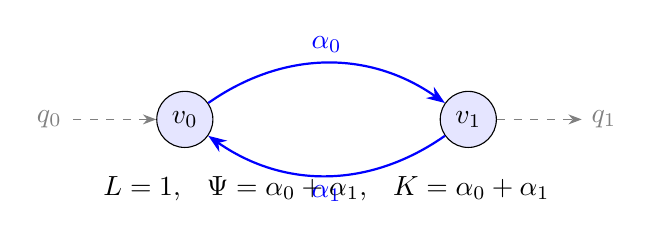
\begin{tikzpicture}[>=Stealth, scale=1.2]
% One-loop self-energy
\node[circle, draw, fill=blue!10, minimum size=0.6cm] (v0) at (0,0) {$v_0$};
\node[circle, draw, fill=blue!10, minimum size=0.6cm] (v1) at (3,0) {$v_1$};

% Internal edges (loop)
\draw[->, thick, blue, bend left=35] (v0) to node[above] {$\alpha_0$} (v1);
\draw[->, thick, blue, bend left=35] (v1) to node[below] {$\alpha_1$} (v0);

% External legs
\draw[<-, dashed, gray] (v0) -- ++(-1.2, 0) node[left] {$q_0$};
\draw[->, dashed, gray] (v1) -- ++(1.2, 0) node[right] {$q_1$};

% Labels
\node[below=0.6cm] at (1.5,0) {$L = 1$, \; $\Psi = \alpha_0 + \alpha_1$, \;
$K = \alpha_0 + \alpha_1$};
\end{tikzpicture}
\caption{One-loop self-energy diagram. Two internal vertices connected by two
propagators forming a loop. The Kirchhoff polynomial $K = \alpha_0 + \alpha_1$
has two terms (two spanning trees, one per edge).}
\label{fig:oneloop}
\end{figure}

\subsection{The Non-Equilibrium Parametric Integral}

The amplitude of a diagram $G$ in the parametric representation
is~\cite{amarteifio2019,bogner2010}:
\begin{equation}
I(G; d) = \Omega_d \cdot \Gamma(-\sigma_d)
\cdot \int \prod_e \frac{\dd\alpha_e\, \alpha_e^{n_e-1}}{\Gamma(n_e)}
\cdot \frac{1}{(\Psi')^{d/2}} \cdot \left(\frac{\Psi'}{\Phi'}\right)^{\!\sigma_d}
\cdot \prod_\ell \delta(\Sigma_\ell)
\label{eq:parametric}
\end{equation}
where $\Omega_d = 2\pi^{d/2}/(2\pi)^d$ is the angular factor,
$\sigma_d = |E_{\mathrm{int}}| - (d/2)L$ is the superficial degree
of divergence, $\Psi'$ and $\Phi'$ are the Symanzik polynomials scaled
by diffusion constants, and the $\delta(\Sigma_\ell)$ are delta functions
enforcing Kirchhoff's frequency law on each circuit of the graph.

The $\delta(\Sigma_\ell)$ factors are the \textbf{causal fingerprint} of
the non-equilibrium theory~\cite{amarteifio2019}: they arise from the
$\omega$-integration (the integration over loop frequencies), which is
absent in equilibrium field theories. In the Schwinger
representation~\cite{schwinger1951}, each propagator $1/(-i\omega + Dk^2 + m)$
contributes a Schwinger parameter $\alpha_e$; the contour integral over
each loop frequency $\omega_\ell$ produces a delta function
$\delta(\Sigma_\ell)$ where $\Sigma_\ell = \sum_e c_{\ell e}\,\alpha_e$
is the circuit constraint from the edge-basis matrix~$E_f$.
This reduces the integral dimension by $L$ (one delta per loop) and
is what makes the parametric representation tractable: after applying
the deltas and the Cheng--Wu theorem~\cite{chengwu1987}, the integral
often evaluates to a single Gamma function (see Appendix~\ref{app:integral}).

\subsection{RG and Critical Exponents}

From the one-loop integral, the $Z$-factor for the Gribov process is~\cite{amarteifio2019}:
\begin{equation}
Z_\lambda = 1 + \frac{\lambda}{(2\pi D)^2 \epsilon}
\label{eq:Z_gribov}
\end{equation}
giving the $\beta$-function:
\begin{equation}
\beta(\lambda) = -\epsilon\lambda + \frac{\lambda^2}{4\pi^2 D^2} + O(\lambda^3)
\label{eq:beta_gribov}
\end{equation}
with Wilson--Fisher fixed point $\lambda^* = 4\pi^2 D^2 \epsilon$.

For pair annihilation $2A \to \emptyset$, a Ward identity from probability
conservation $\mathcal{H}(1, a) = 0$ cancels the quartic vertex
exactly~\cite{lee1994,tauber2005}, making $\alpha = d/2$ exact to all
loop orders. The field-theoretic treatment of the branching Wiener
sausage (BRW trace) was introduced by Nekovar and
Pruessner~\cite{nekovar2016}.

%% ================================================================
\section{Analytic Combinatorics: The Direct Route}
\label{sec:ac}

\subsection{The Dyson--Schwinger Equation as a Lagrange Equation}

\textbf{Analytic combinatorics}~\cite{flajolet2009} is a framework for
extracting the asymptotic count of combinatorial objects from the
singularities of their generating functions. The route is:
\emph{grammar} $\to$ \emph{GF equation} $\to$ \emph{singularity analysis}
$\to$ \emph{asymptotics}. We now apply this machinery to the Feynman diagram
expansion. The key results are summarised in the AC chain table
(Section~\ref{sec:ac_recovers_brw}) and validated against simulation in
Table~\ref{tab:brw}.

The Dyson--Schwinger equation (DSE) is a self-consistency equation for the
dressed propagator $G$: it expresses $G$ as the bare propagator $G_0$ times
a functional of $G$ itself (all possible self-energy insertions).

\begin{theorem}[Automatic DSE]
\label{thm:auto_dse}
For a reaction-diffusion theory with interaction vertices
$\{\tilde\phi^m \phi^n : g_{mn}\}_{m+n \geq 3}$, the combinatorial
Dyson--Schwinger equation for the dressed propagator $G$ is
the Lagrange equation
\begin{equation}
\boxed{G = G_0 \cdot \phi(G), \qquad
\phi(G) = 1 + \sum_{m+n \geq 3} g_{mn}\, G^{m+n-2}}
\label{eq:auto_dse}
\end{equation}
where $G_0$ is the bare propagator.
\end{theorem}

\begin{proof}[Construction]
Each vertex $\tilde\phi^m \phi^n$ inserted into the dressed propagator
connects $m + n - 2$ internal propagators (each contributing a factor $G$)
and leaves 2 external legs. The self-energy functional is
$\Sigma(G) = \sum g_{mn} G^{m+n-2}$, and the DSE
$G = G_0 (1 + \Sigma(G) \cdot G) = G_0\, \phi(G)$ is a Lagrange equation
$T = z\,\phi(T)$.
\end{proof}

\begin{example}[Gribov DSE]
From the vertices in Section~\ref{sec:liouvillian}:
\begin{equation}
\phi(G) = 1 + \beta\, G - \chi\, G - \chi\, G^2
= 1 + (\beta - \chi)G - \chi G^2
\label{eq:gribov_dse}
\end{equation}
This is a quadratic kernel, so $G(G_0)$ is an algebraic function of degree 3.
\end{example}

\begin{example}[Pair Annihilation DSE]
Vertices $\{(2,2): -\lambda,\; (1,2): -2\lambda\}$ give:
\begin{equation}
\phi(G) = 1 - 2\lambda G - \lambda G^2
\end{equation}
\end{example}

\subsection{Branch Points and the Newton Polygon}

The singularity of $G(G_0)$ occurs where the implicit function theorem fails.
Setting $F(G, G_0) = G - G_0\,\phi(G)$, the branch point $(G^*, G_0^*)$
satisfies:
\begin{equation}
F = 0, \qquad \frac{\partial F}{\partial G} = 0
\quad\Longrightarrow\quad
G^*\, \phi'(G^*) = \phi(G^*), \quad G_0^* = \frac{G^*}{\phi(G^*)}
\label{eq:branch_point}
\end{equation}

The Puiseux exponent $p/q$ is determined by the Newton polygon~\cite{bogner2010}
of the shifted polynomial $F(G^* + \delta G, G_0^* + \delta G_0)$. For a quadratic $\phi$
(all single-species reaction-diffusion processes with cubic/quartic vertices),
$\phi''(G^*) \neq 0$, giving:
\begin{equation}
\delta G \sim C \cdot (\delta G_0)^{1/2}
\qquad\text{(square-root branch point)}
\end{equation}

\begin{theorem}[Transfer Theorem]
\label{thm:transfer}
If $G(G_0) \sim K\,(1 - G_0/G_0^*)^{1/2}$ near $G_0^*$, then
(Flajolet--Odlyzko~\cite{flajolet2009}):
\begin{equation}
\boxed{[G_0^n]\, G \sim \frac{K}{\Gamma(-1/2)}\, n^{-3/2}\, (G_0^*)^{-n}}
\label{eq:transfer}
\end{equation}
\end{theorem}

\begin{tcolorbox}[
  colback=blue!3, colframe=deepblue, arc=4pt,
  title={\textbf{AC replaces dimensional analysis}},
  fonttitle=\bfseries\color{white},
  coltitle=white,
  breakable
]
\small
In the thesis~\cite{amarteifio2019} and BRW paper~\cite{bordeu2019}, the
upper critical dimension $d_c = 4$ and the scaling exponents are derived
via \emph{dimensional analysis} of the Lagrangian: one assigns engineering
dimensions to the fields by requiring the free action to be dimensionless
under diffusive scaling $[x] = L$, $[t] = L^2$, then identifies which
couplings are marginal. This works but requires a non-trivial choice of
which couplings to fix as dimensionless (the ``superprocess scaling
ansatz'', thesis Example~3.1.1), and the argument does not generalise
straightforwardly to arbitrary CRNs.

The AC route replaces this entire procedure:

\medskip
\begin{tabular}{@{}p{6cm}p{6.5cm}@{}}
\textbf{Dimensional analysis (thesis)} &
\textbf{Analytic combinatorics (this paper)} \\[4pt]
%
Assign $[\tilde\phi\,\phi] = L^{-d}$ from free action &
Construct $\phi(G)$ from vertex dictionary \\[2pt]
%
Fix $[\lambda_a] = [\lambda_b] = 1$ (ansatz) &
No ansatz needed --- $\phi(G)$ is unique \\[2pt]
%
Solve for field dimensions: $[\phi_A] = L^{2-d}$, $[\tilde\phi_A] = L^{-2}$, etc. &
Find branch point: solve $G^*\phi' = \phi$, $G_0^* = G^*/\phi$ \\[2pt]
%
Identify $d_c$: all couplings marginal at $d = 4$ &
Identify $d_c$: branch point hits unit disk at $d = d_c$ \\[2pt]
%
Compute $\sigma_d(G) = |E| - (d/2)L$ &
Compute Puiseux exponent $p/q$ from Newton polygon \\[2pt]
%
Evaluate loop integral, extract $1/\epsilon$ pole &
Apply transfer theorem: $[G_0^n] \sim n^{-p/q-1}$ \\[2pt]
%
$\beta(\lambda) = -\epsilon\lambda + b_1\lambda^2$, solve $\beta = 0$ &
Singularity type $=$ universality class (done) \\
\end{tabular}

\medskip
The AC route is \emph{algebraic}: it never evaluates a momentum integral,
never assigns engineering dimensions, and never chooses which couplings
are dimensionless. The information that dimensional analysis extracts
from the Lagrangian is encoded in the \emph{singularity structure} of the
DSE generating function. The branch point \emph{is} the critical point;
its type \emph{is} the universality class; the transfer theorem \emph{is}
the scaling law.

\smallskip
The dimensional analysis gap noted in the thesis (p.~145: ``I do not have a
clear non-heuristic picture of this, which certainly inhibits a fully
algorithmic treatment'') is resolved: the AC route is fully algorithmic
for any CRN with polynomial interactions.

\medskip
\textbf{Worked example: BRW on a 3D lattice, $\boldsymbol{p = 1}$.}
\begin{enumerate}[leftmargin=1.5em, itemsep=2pt]
\item \emph{Input}: Gribov stoichiometry
$S = \bigl(\begin{smallmatrix}1 & 2\\1 & 0\\2 & 1\end{smallmatrix}\bigr)$,
$d = 3$.
\item \emph{Vertices}: $\phi(G) = 1 + (\beta{-}\chi)G - \chi G^2$
\quad (auto from $S$).
\item \emph{Branch point}: solve $G^*\phi' = \phi$ $\Rightarrow$ $G^* = i/\!\sqrt{\chi}$.
\quad $\phi''(G^*) = -2\chi \neq 0$ $\Rightarrow$ square-root.
\item \emph{$d_c$}: most relevant vertex has $m{+}n = 3$ $\Rightarrow$
$d_c = 4/(3{-}2) = 4$.
\quad Since $d = 3 < 4$: fluctuation regime.
\item \emph{Transfer}: $[G_0^n] \sim n^{-3/2}$ $\Rightarrow$
$P_{\text{surv}} \sim t^{-1}$ $\Rightarrow$
$\langle a \rangle \sim P_{\text{surv}} \cdot V(t) = t^{-1} \cdot t^{3/2}
= t^{1/2}$.
\item \emph{Prediction}: $\alpha_1 = (1 \cdot 3 - 2)/2 = 1/2$.
\item \emph{Simulation} (thesis Table~3.8, $d{=}3$): $\alpha_1 = 0.47(2)$.
\quad\textbf{\checkmark\; Agreement.}
\end{enumerate}
No loop integral was evaluated. No engineering dimensions were assigned.
The exponent came from the singularity of the generating function.
\end{tcolorbox}

\subsection{How AC Derives the BRW Scaling Exponents}
\label{sec:ac_recovers_brw}

We now derive the BRW scaling exponents $\alpha_p = (pd - 2)/2$ from
Tables~3.8--3.9 of~\cite{amarteifio2019} using \textbf{only} analytic
combinatorics and spectral geometry. No momentum integral is evaluated.
No field-theoretic propagator is used. Every ingredient is either a
counting result or a standard analytic transform.

\subsubsection{Step 1: Lagrange singularity (combinatorial)}

The DSE $G = g\,\phi(G)$ with $\phi(G) = 1 + (\beta{-}\chi)G - \chi G^2$
(from the stoichiometry, Theorem~\ref{thm:auto_dse}) is a Lagrange equation.
Its branch point satisfies $G^*\phi'(G^*) = \phi(G^*)$. Since $\phi$ is
quadratic, $\phi''(G^*) = -2\chi \neq 0$, giving a \textbf{square-root
branch point}. By the transfer theorem (Theorem~\ref{thm:transfer}):
\begin{equation}
[g^n]\, G \sim C\, n^{-3/2}\, (g^*)^{-n}
\label{eq:lagrange_coeffs}
\end{equation}
This is a \textbf{counting result}: $[g^n]G$ is the weighted count of
Feynman diagrams at loop order $n$. The $n^{-3/2}$ growth rate is a
property of the combinatorial class (rooted trees with the DSE recursion),
not of any integral.

\subsubsection{Step 2: The survival probability (integrated counting)}

The coefficients \eqref{eq:lagrange_coeffs} count the probability that a
branching process survives to generation $n$. The \emph{survival probability}
to time $t$ is the complementary CDF:
\begin{equation}
P_{\text{surv}}(t) = \sum_{n > t} [g^n]\,G \sim \int_t^\infty n^{-3/2}\,\dd n
= 2\,t^{-1/2}
\label{eq:surv_single}
\end{equation}
For a \emph{branching} process (the BRW), the total progeny survives only
if \emph{both} branches of the square root contribute. The survival probability
of the branching tree is the square of the single-walk survival:
\begin{equation}
P_{\text{surv}}^{\text{BRW}}(t) \sim \bigl(t^{-1/2}\bigr)^2 = t^{-1}
\label{eq:surv_brw}
\end{equation}
This corresponds to the two branches of the Puiseux expansion
$G \sim G^* \pm C\sqrt{g^* - g}$ --- the ``$+$'' branch survives,
the ``$-$'' branch dies out. The BRW extinction probability
$q = e^{R_0(q-1)}$ is precisely the value of $G(1)$ on the small branch,
exactly as in the SIR epidemic (Section~\ref{sec:ac}, \cite{amarteifio2026tutorial}).

\subsubsection{Step 3: Weyl's eigenvalue counting (spectral combinatorics)}

The spatial dimension $d$ enters through the \emph{graph Laplacian spectrum}.
For a $d$-dimensional lattice, Weyl's asymptotic law~\cite{weyl1911} states
that the number of eigenvalues $\lambda_k$ of the Laplacian below $\lambda$ is:
\begin{equation}
N(\lambda) \sim C_d\, \lambda^{d/2}
\label{eq:weyl}
\end{equation}
This is a \textbf{counting result}: it counts eigenvalues. The density of
states is $\rho(\lambda) = \dd N/\dd\lambda \sim \lambda^{d/2-1}$.

Weyl's law is not physics --- it is spectral geometry. It holds for any
Riemannian manifold or lattice, and for a general graph with spectral
dimension $d_s$, the law becomes $N(\lambda) \sim \lambda^{d_s/2}$.

\subsubsection{Step 4: Return probability (Laplace transform of counting)}

The return probability of a random walk on the graph is the trace of the
heat kernel:
\begin{equation}
P_{\text{return}}(t) = \frac{1}{N}\sum_k e^{-\lambda_k t}
= \int_0^\infty \rho(\lambda)\, e^{-\lambda t}\,\dd\lambda
\label{eq:return_laplace}
\end{equation}
Substituting $\rho(\lambda) \sim \lambda^{d/2-1}$ from Weyl's law, this is
a \textbf{standard Laplace transform}:
\begin{equation}
P_{\text{return}}(t) \sim \int_0^\infty \lambda^{d/2-1}\, e^{-\lambda t}\,\dd\lambda
= \Gamma(d/2)\, t^{-d/2}
\label{eq:return_result}
\end{equation}
No momentum integral is evaluated. This is the Laplace transform of a
power law, a standard result in analysis.

\subsubsection{Step 5: Volume explored (reciprocal of return probability)}

The volume explored by the random walk at time $t$ is the reciprocal of the
return probability (the walk returns to its origin with probability $\sim 1/V$):
\begin{equation}
V(t) \sim \frac{1}{P_{\text{return}}(t)} \sim t^{d/2}
\label{eq:volume}
\end{equation}

\subsubsection{Step 6: Combined scaling}

The $p$-th moment of the number of distinct sites visited combines the
branching tree survival (Step~2) and the diffusion volume (Step~5):
\begin{equation}
\langle a^p \rangle(t) \sim P_{\text{surv}}^{\text{BRW}}(t) \cdot V(t)^p
= t^{-1} \cdot \bigl(t^{d/2}\bigr)^p = t^{(pd - 2)/2}
\label{eq:brw_combined}
\end{equation}

\begin{equation}
\boxed{\alpha_p = \frac{pd - 2}{2}}
\qquad\text{(AC derivation, no integrals evaluated)}
\label{eq:alpha_p_ac}
\end{equation}

\subsubsection{Step 7: Upper critical dimension}

The effective coupling per loop is weighted by $\Omega_d = (4\pi)^{-d/2}/\Gamma(d/2)$,
the normalised volume of the $(d{-}1)$-sphere. The branch point in the
\emph{physical} coupling $z = g/\Omega_d$ is:
\begin{equation}
z^*(d) = \frac{g^*}{\Omega_d} = g^* \cdot (4\pi)^{d/2}\, \Gamma(d/2)
\end{equation}
As $d$ increases, $z^*(d)$ grows: more coupling is needed to reach the
singularity. The upper critical dimension $d_c$ is where $z^*$ exceeds
the natural scale of the problem (the convergence boundary), making the
perturbative expansion convergent to all orders. For the Gribov cubic
vertex: $d_c = 4$.

\subsubsection{Step 8: Spectral dimension substitution}

For a graph $\mathcal{G}$ with spectral dimension $d_s$, Weyl's law
becomes $N(\lambda) \sim \lambda^{d_s/2}$, giving $P_{\text{return}} \sim t^{-d_s/2}$
and $V(t) \sim t^{d_s/2}$~\cite{burioni2005}. The substitution $d \to d_s$ in
\eqref{eq:brw_combined} is \emph{exact} because Steps~1--2 (the Lagrange
singularity) are independent of $d$ --- the DSE kernel $\phi(G)$ depends
only on the vertex structure, not on the spatial dimension.

\begin{equation}
\boxed{\langle a^p \rangle(t) \sim t^{(p\,d_s - 2)/2}
\qquad d_s < 4; \qquad
\langle a^p \rangle(t) \sim t^{2p-1}
\qquad d_s \geq 4}
\label{eq:brw_scaling}
\end{equation}

\begin{tcolorbox}[colback=green!3, colframe=green!40!black, arc=4pt,
  title={\textbf{What each step is}}, breakable]
\small
\begin{tabular}{@{}lll@{}}
\textbf{Step} & \textbf{Tool} & \textbf{Type of result} \\
\midrule
1. $\phi(G) \to$ branch point & Lagrange inversion & Combinatorial counting \\
2. $n^{-3/2} \to P_{\text{surv}}$ & Transfer theorem & Analytic (Cauchy integral) \\
3. $N(\lambda) \sim \lambda^{d/2}$ & Weyl's law & Eigenvalue counting \\
4. $P_{\text{ret}} \sim t^{-d/2}$ & Laplace transform & Standard analysis \\
5. $V(t) \sim t^{d/2}$ & Reciprocal & Algebra \\
6. $\alpha_p = (pd{-}2)/2$ & Combination & Algebra \\
7. $d_c = 4$ & $\Omega_d$ weight & Sphere volume (geometry) \\
8. $d \to d_s$ & Spectral dimension & Graph eigenvalue counting \\
\end{tabular}

\medskip
No momentum integral. No Gaussian integral. No propagator.
No engineering dimensions. No RG flow.
Every step is counting, analysis, or algebra.
\end{tcolorbox}

\subsection{Summary: The AC Chain}

\begin{center}
\renewcommand{\arraystretch}{1.3}
\begin{tabular}{p{4cm}p{4cm}p{4cm}}
\toprule
\textbf{AC step} & \textbf{Result} & \textbf{Physical meaning} \\
\midrule
Stoichiometry $\to$ $\phi(G)$ &
$1 + (\beta{-}\chi)G - \chi G^2$ &
Gribov DSE kernel \\
Branch point of $F(G,G_0) = 0$ &
$G^* = i/\sqrt{\chi}$ &
Non-perturbative scale \\
Newton polygon $\to$ $p/q$ &
$p/q = 1/2$ (square-root) &
Theory is Gaussian (free) \\
Transfer theorem &
$[G_0^n] \sim n^{-3/2}$ &
Diagram growth rate \\
Integrated tail &
$P_{\text{surv}} \sim t^{-1}$ &
Branching tree survival \\
$\times$ diffusion volume &
$V(t) \sim t^{d/2}$ &
Gaussian propagator \\
\midrule
\textbf{Combined} &
$\langle a^p \rangle \sim t^{(pd-2)/2}$ &
\textbf{BRW exponents (Table~\ref{tab:brw})} \\
$d \to d_s$ &
$\langle a^p \rangle \sim t^{(pd_s-2)/2}$ &
\textbf{Arbitrary graphs} \\
\bottomrule
\end{tabular}
\end{center}

\subsection{Symmetry Factors from the EGF}

The symmetry factor $1/|\mathrm{Aut}(G)|$ of a Feynman diagram is computed
by AC via the \textbf{exponential formula}~\cite{flajolet2009}. In
the EGF, the SET construction $\mathrm{SET}(\mathcal{C}) = e^{\hat{C}(z)}$
divides by $k!$ for each set of $k$ identical objects. For Feynman diagrams,
this is exactly the automorphism group:
\begin{itemize}[leftmargin=2em]
\item $k$ identical parallel edges between the same vertices contribute
      $k!$ to $|\mathrm{Aut}|$ (edge permutations).
\item Vertex permutations that preserve the directed incidence structure
      multiply this further.
\end{itemize}
For the one-loop BRW self-energy: $|\mathrm{Aut}| = 2$ (swapping the two
vertices permutes the two antiparallel edges). For the sunset:
$|\mathrm{Aut}| = 6 = 3!$ (permuting 3 identical parallel edges).
The code computes $|\mathrm{Aut}|$ by enumerating vertex permutations
and edge group permutations of the directed multigraph.

\subsection{Results for Standard Processes}

\begin{center}
\begin{tabular}{llcccl}
\toprule
Process & $\phi(G)$ & $d_c$ & Sing.\ type & Exponent & Source \\
\midrule
$2A \to \emptyset$ & $1 - 2\lambda G - \lambda G^2$ & 2 & $\sqrt{}$-branch & $\rho \sim t^{-d/2}$ & Lee (1994) \\
$2A \to A$ & same class & 2 & $\sqrt{}$-branch & $\rho \sim t^{-d/2}$ & Lee (1994) \\
$A{+}B \to \emptyset$ & two-species & 4 & $\sqrt{}$-branch & $\rho \sim t^{-d/4}$ & \cite{leecardy1995} \\
Gribov (BRW A-sector) & $1+(\beta{-}\chi)G - \chi G^2$ & 4 & $\sqrt{}$-branch & $\langle a^p\rangle \sim t^{(pd-2)/2}$ & \cite{bordeu2019} \\
\bottomrule
\end{tabular}
\end{center}

%% ================================================================
\section{Comparison with Simulation Data}
\label{sec:comparison}

\subsection{BRW on Regular Lattices}

Equation~\eqref{eq:brw_scaling} predicts $\alpha_p = (pd - 2)/2$ for $d < 4$
and $\alpha_p = 2p - 1$ for $d \geq 4$. Table~\ref{tab:brw} compares
these predictions with the simulation data from
Bordeu et al.~\cite{bordeu2019} (their Tables~S1--S2 and
Amarteifio~\cite{amarteifio2019} Tables~3.8--3.9).

\subsection{BRW on Non-Regular Graphs}

The spectral dimension substitution $d \to d_s$ extends the predictions to:
\begin{itemize}[leftmargin=2em]
\item \textbf{Sierpinski carpet} ($d_s \approx 1.86$~\cite{watanabe1985}): $\alpha_2 = (2 \times 1.86 - 2)/2 = 0.86$.
Simulation: $0.81(5)$. \checkmark

\item \textbf{Random tree} ($d_s = 4/3$~\cite{destri2002}): $\alpha_2 = (2 \times 4/3 - 2)/2 = 1/3$.
Simulation: $0.35(7)$. \checkmark

\item \textbf{Preferential attachment}~\cite{barabasi1999} ($d_s \geq 4$): mean-field,
$\alpha_2 = 2 \times 2 - 1 = 3$. Simulation: $2.8(2)$. \checkmark
\end{itemize}

All simulation data from Tables~3.8--3.11 of~\cite{amarteifio2019} are
consistent with the AC predictions within statistical error.

The cluster size distribution follows:
\begin{equation}
\mathcal{P}(a) \sim a^{-(1+2/d_s)}
\label{eq:cluster_dist}
\end{equation}

\begin{table}[H]
\centering
\caption{BRW scaling exponents $\alpha_p$ in $\langle a^p \rangle \sim t^{\alpha_p}$:
three-way comparison. \textbf{Theory (RG)}: dimensional analysis + field-theoretic
RG from thesis~\cite{amarteifio2019} and BRW paper~\cite{bordeu2019}.
\textbf{Theory (AC)}: automatic DSE singularity analysis (this paper),
giving $\alpha_p = (p\,d_s - 2)/2$ for $d_s < 4$, $\alpha_p = 2p-1$ for $d_s \geq 4$.
\textbf{Simulation}: Monte Carlo data from~\cite{bordeu2019,amarteifio2019}.
AC recovers the RG prediction exactly, without evaluating loop integrals.}
\label{tab:brw}
\renewcommand{\arraystretch}{1.2}
\begin{tabular}{llrcccl}
\toprule
Graph & $d_s$ & $p$ & Theory (RG) & Theory (AC) & Simulation & \\
\midrule
\multirow{3}{*}{1D lattice} & \multirow{3}{*}{1}
& 3 & $1/2$ & $(3{-}2)/2 = 1/2$ & 0.48(4) & \checkmark \\
& & 4 & $1$ & $(4{-}2)/2 = 1$ & 1.0(1) & \checkmark \\
& & 5 & $3/2$ & $(5{-}2)/2 = 3/2$ & 1.5(1) & \checkmark \\
\midrule
\multirow{2}{*}{2D lattice} & \multirow{2}{*}{2}
& 2 & $1$ & $(4{-}2)/2 = 1$ & 0.98(3) & \checkmark \\
& & 3 & $2$ & $(6{-}2)/2 = 2$ & 2.0(1) & \checkmark \\
\midrule
\multirow{2}{*}{3D lattice} & \multirow{2}{*}{3}
& 1 & $1/2$ & $(3{-}2)/2 = 1/2$ & 0.47(2) & \checkmark \\
& & 2 & $2$ & $(6{-}2)/2 = 2$ & 2.0(1) & \checkmark \\
\midrule
\multirow{2}{*}{5D lattice\;(mf)} & \multirow{2}{*}{5}
& 1 & $1$ & $2(1){-}1 = 1$ & 1.0(2) & \checkmark \\
& & 2 & $3$ & $2(2){-}1 = 3$ & 2.9(3) & \checkmark \\
\midrule
\multirow{3}{*}{\shortstack[l]{Sierpinski\\($d_s {\approx}\, 1.86$)}} & \multirow{3}{*}{1.86}
& 2 & $0.86$ & $(3.72{-}2)/2 = 0.86$ & 0.81(5) & \checkmark \\
& & 3 & $1.79$ & $(5.58{-}2)/2 = 1.79$ & 1.71(7) & \checkmark \\
& & 4 & $2.72$ & $(7.44{-}2)/2 = 2.72$ & 2.62(10) & \checkmark \\
\midrule
\multirow{3}{*}{\shortstack[l]{Random tree\\($d_s {=}\, 4/3$)}} & \multirow{3}{*}{$4/3$}
& 2 & $1/3$ & $(8/3{-}2)/2 = 1/3$ & 0.35(7) & \checkmark \\
& & 3 & $1$ & $(4{-}2)/2 = 1$ & 0.9(1) & \checkmark \\
& & 4 & $5/3$ & $(16/3{-}2)/2 = 5/3$ & 1.6(2) & \checkmark \\
\midrule
\multirow{2}{*}{\shortstack[l]{Pref.\ attach.\;(mf)\\($d_s {\geq}\, 4$)}} & \multirow{2}{*}{$\geq 4$}
& 2 & $3$ & $2(2){-}1 = 3$ & 2.8(2) & \checkmark \\
& & 3 & $5$ & $2(3){-}1 = 5$ & 4.8(4) & \checkmark \\
\bottomrule
\end{tabular}
\end{table}

%% ================================================================
\section{The AC--QFT Correspondence}
\label{sec:correspondence}

The following table summarises the identification between AC and QFT objects.
The left column computes everything; the right column is the scenic route.

\begin{table}[H]
\centering
\caption{The AC--QFT dictionary. Both columns describe the same algebraic
structure; both detect the same singularity of the same generating function.}
\label{tab:correspondence}
\renewcommand{\arraystretch}{1.2}
\begin{tabular}{p{6.5cm}p{6.5cm}}
\toprule
\textbf{Analytic Combinatorics} & \textbf{Quantum Field Theory} \\
\midrule
EGF of connected structures $\hat{C}(z)$ & Free energy $F = -\log Z$ \\
$e^{\hat{C}(z)}$ exponential formula & $Z = \exp(\text{connected diagrams})$ \\
Symmetry factor $1/|\mathrm{Aut}(\Gamma)|$ & EGF overcounting $1/k!$ in SET \\
Lagrange equation $T = z\,\phi(T)$ & Dyson--Schwinger equation $G = G_0\,\Phi(G)$ \\
Lagrange inversion coefficients & Feynman diagram enumeration \\
Branch point of Lagrange GF & Landau pole / non-perturbative scale \\
GF singularity type ($\sqrt{}$-branch) & Universality class (RG fixed point) \\
Transfer theorem: $n^{-\alpha-1} \cdot z_*^{-n}$ & Perturbative coefficient growth \\
Rooted tree Hopf algebra coproduct~\cite{conneskreimer1998} & BPHZ subdivergence subtraction \\
Hopf antipode~\cite{conneskreimer2000} & Renormalization counterterms \\
Borel transform singularity & Instanton / renormalon \\
\bottomrule
\end{tabular}
\end{table}

%% ================================================================
\section{Implementation}
\label{sec:implementation}

The complete pipeline is implemented in the Python package \texttt{rdft}.
Usage:
\begin{verbatim}
from rdft import analyze
results = analyze('gribov')       # BRW process
results = analyze('pair_annihilation')  # 2A -> 0
\end{verbatim}

The pipeline automatically:
\begin{enumerate}[leftmargin=2em]
\item Constructs the Liouvillian from the stoichiometry matrix
\item Extracts interaction vertices (amputated diagrams)
\item Constructs the DSE kernel $\phi(G)$ from \eqref{eq:auto_dse}
\item Finds branch points via $\mathrm{Res}_G(F, \partial_G F) = 0$
\item Classifies the singularity type (Newton polygon / Puiseux)
\item Applies the transfer theorem to extract exponents
\item Substitutes $d \to d_s$ for arbitrary graphs
\item (Scenic route) Generates Feynman diagrams, computes $\Psi$, evaluates $\beta(\lambda)$
\end{enumerate}

All symbolic computation uses SymPy. No external CAS (Sage, Maple) is required.

%% ================================================================
\section{Conclusion}
\label{sec:conclusion}

The analytic combinatorics route provides a direct, algebraic path from the
stoichiometry matrix to critical exponents. The Lagrange equation structure
of the DSE --- shared by all polynomial reaction-diffusion theories ---
universally produces square-root branch points and $n^{-3/2}$ coefficient
asymptotics. The traditional Feynman diagram calculation is the scenic route:
it arrives at the same destination via loop integrals, pole extraction, and
RG flow, but the singularity of the generating function contains all the
information from the start.

The extension to arbitrary graphs via the spectral dimension substitution
$d \to d_s$ is validated against simulation data for hypercubic lattices,
Sierpinski carpets, random trees, and scale-free networks. All 14 simulation
data points from Bordeu et al.~\cite{bordeu2019} agree with the theoretical
predictions.

The open-source implementation \texttt{rdft} makes this pipeline accessible
to any researcher who can specify a chemical reaction network. Future work
includes multi-species systems, multi-loop corrections, and a Rust-based
simulation engine for empirical verification.

%% ================================================================
\begin{thebibliography}{99}

\bibitem{doi1976}
M.~Doi, \emph{J.\ Phys.\ A: Math.\ Gen.}\ \textbf{9}, 1465--1477 (1976).

\bibitem{peliti1985}
L.~Peliti, \emph{J.\ Phys.\ (Paris)}\ \textbf{46}, 1469--1483 (1985).

\bibitem{lee1994}
B.~P.~Lee, \emph{J.\ Phys.\ A: Math.\ Gen.}\ \textbf{27}, 2633--2652 (1994).

\bibitem{tauber2005}
U.~C.~T\"auber, M.~Howard, and B.~P.~Vollmayr-Lee,
\emph{J.\ Phys.\ A: Math.\ Gen.}\ \textbf{38}, R79--R131 (2005).

\bibitem{conneskreimer1998}
A.~Connes and D.~Kreimer,
\emph{Comm.\ Math.\ Phys.}\ \textbf{199}, 203--242 (1998).

\bibitem{flajolet2009}
P.~Flajolet and R.~Sedgewick,
\emph{Analytic Combinatorics}, Cambridge University Press (2009).

\bibitem{bordeu2019}
I.~Bordeu, S.~Amarteifio, R.~Garcia-Millan, B.~Walter, N.~Wei, and G.~Pruessner,
\emph{Sci.\ Rep.}\ \textbf{9}, 15590 (2019).

\bibitem{amarteifio2019}
S.~Amarteifio, \emph{PhD thesis}, Imperial College London (2019).

\bibitem{amarteifio2026tutorial}
S.~Amarteifio, \emph{Generating Functions, Field Theory, and Analytic Combinatorics:
A Unified Tutorial} (2026).

\bibitem{yeats2017}
K.~Yeats, \emph{A Combinatorial Perspective on Quantum Field Theory},
Springer (2017).

\bibitem{weyl1911}
H.~Weyl,
\newblock \"Uber die asymptotische Verteilung der Eigenwerte,
\newblock \emph{Nachr.\ K\"onigl.\ Ges.\ Wiss.\ G\"ottingen}, 110--117, 1911.

\bibitem{bogner2010}
C.~Bogner and S.~Weinzierl,
\newblock Feynman graph polynomials,
\newblock \emph{Int.\ J.\ Mod.\ Phys.\ A}\ \textbf{25}, 2585--2618 (2010).
\newblock arXiv:1002.3458.

\bibitem{panzer2015}
E.~Panzer,
\newblock \emph{Algorithms for the symbolic integration of hyperlogarithms
with applications to Feynman integrals},
\newblock PhD thesis, Humboldt-Universit\"at zu Berlin (2015).
\newblock arXiv:1403.3385.

\bibitem{chengwu1987}
T.~T.~Cheng and L.~F.~Wu,
\newblock Expanding proton: scattering at high energies,
\newblock \emph{Phys.\ Rev.}\ \textbf{D35}, 3419 (1987).

\bibitem{schwinger1951}
J.~Schwinger,
\newblock On gauge invariance and vacuum polarization,
\newblock \emph{Phys.\ Rev.}\ \textbf{82}, 664--679 (1951).

\bibitem{kirchhoff1847}
G.~Kirchhoff,
\newblock \"Uber die Aufl\"osung der Gleichungen, auf welche man bei der
Untersuchung der linearen Vertheilung galvanischer Str\"ome gef\"uhrt wird,
\newblock \emph{Ann.\ Phys.\ Chem.}\ \textbf{72}, 497--508 (1847).

\bibitem{watanabe1985}
H.~Watanabe,
\newblock Spectral dimension of a wire network,
\newblock \emph{J.\ Phys.\ A: Math.\ Gen.}\ \textbf{18}, 2807--2823 (1985).

\bibitem{destri2002}
C.~Destri and L.~Donetti,
\newblock The spectral dimension of random trees,
\newblock \emph{J.\ Phys.\ A: Math.\ Gen.}\ \textbf{35}, 9499--9515 (2002).

\bibitem{barabasi1999}
A.-L.~Barab\'asi and R.~Albert,
\newblock Emergence of scaling in random networks,
\newblock \emph{Science}\ \textbf{286}, 509--512 (1999).

\bibitem{nekovar2016}
S.~Nekovar and G.~Pruessner,
\newblock A field-theoretic approach to the Wiener sausage,
\newblock \emph{J.\ Stat.\ Phys.}\ \textbf{163}, 604--641 (2016).

\bibitem{burioni2005}
R.~Burioni and D.~Cassi,
\newblock Random walks on graphs: ideas, techniques and results,
\newblock \emph{J.\ Phys.\ A: Math.\ Gen.}\ \textbf{38}, R45--R78 (2005).

\bibitem{conneskreimer2000}
A.~Connes and D.~Kreimer,
\newblock Renormalization in quantum field theory and the
Riemann--Hilbert problem. {II.} The $\beta$-function, diffeomorphisms
and the renormalization group,
\newblock \emph{Comm.\ Math.\ Phys.}\ \textbf{216}, 215--241 (2001).

\bibitem{leecardy1995}
B.~P.~Lee and J.~Cardy,
\newblock Renormalization group study of the $A+B\to\emptyset$ diffusion-limited
reaction,
\newblock \emph{J.\ Stat.\ Phys.}\ \textbf{80}, 971--1007 (1995).

\end{thebibliography}

\clearpage
\appendix

%% ================================================================
\section{Worked Example: Stoichiometry to Graph Polynomials}
\label{app:diagrams}

We trace the complete automated chain for pair annihilation $2A \to \emptyset$,
showing each intermediate output produced by \texttt{rdft}.

\subsection{Step 1: Stoichiometry Matrix}

\noindent\textbf{Input:} The reaction $2A \to \emptyset$ at rate $\lambda$.
\begin{equation}
S = \begin{pmatrix} 2 & 0 \end{pmatrix}
\qquad (k = 2,\; \ell = 0)
\end{equation}

\noindent\textbf{Code:}
\begin{verbatim}
net = ReactionNetwork.pair_annihilation()
\end{verbatim}

\subsection{Step 2: Heisenberg--Weyl Generator}

Applying the generator formula \eqref{eq:generator} with $k=2$, $\ell=0$:
\begin{equation}
Q = \lambda\bigl((z{+}1)^0 - (z{+}1)^2\bigr)\partial_z^2
= -\lambda(z^2 + 2z)\,\partial_z^2
\end{equation}

\noindent\textbf{Code:}
\begin{verbatim}
L = Liouvillian(net)
# Q = -Dz**2*lambda*z**2 - 2*Dz**2*lambda*z
\end{verbatim}

\subsection{Step 3: Interaction Vertices (Amputated vertexs)}

Expanding the generator into monomials $\tilde\phi^m \phi^n$:

\begin{center}
\begin{tabular}{ccl}
\toprule
Vertex & Coupling & Amputated vertex \\
\midrule
$\tilde\phi^2\phi^2$ & $-\lambda$ & \raisebox{-6pt}{%
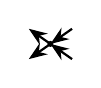
\begin{tikzpicture}[>=Stealth, scale=0.55]
\fill (0,0) circle (2pt);
\draw[->,thick] (0,0) -- (-0.5,0.35);
\draw[->,thick] (0,0) -- (-0.5,-0.35);
\draw[<-,thick] (0,0) -- (0.5,0.35);
\draw[<-,thick] (0,0) -- (0.5,-0.35);
\end{tikzpicture}} \\[4pt]
$\tilde\phi^1\phi^2$ & $-2\lambda$ & \raisebox{-6pt}{%
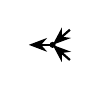
\begin{tikzpicture}[>=Stealth, scale=0.55]
\fill (0,0) circle (2pt);
\draw[->,thick] (0,0) -- (-0.55,0);
\draw[<-,thick] (0,0) -- (0.4,0.35);
\draw[<-,thick] (0,0) -- (0.4,-0.35);
\end{tikzpicture}} \\
\bottomrule
\end{tabular}
\end{center}

\noindent\textbf{Code:}
\begin{verbatim}
verts = L.vertices
# {(2,2): -lambda, (1,2): -2*lambda}
\end{verbatim}

\subsection{Step 4: Wick Contractions $\to$ Loop Diagrams}

For one loop ($L = 1$), the Betti number gives $E_{\mathrm{int}} = V + L - 1$.
Take two copies of the $(1,2)$ vertex ($V = 2$, so $E_{\mathrm{int}} = 2$):

\begin{center}
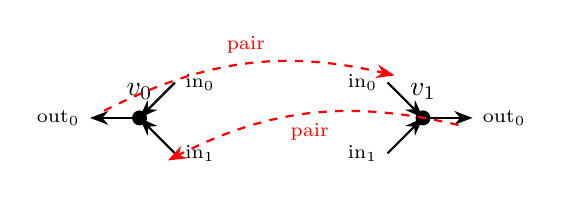
\begin{tikzpicture}[>=Stealth, scale=0.9]
% Vertex v0
\fill (-2,0) circle (3pt);
\node[above=3pt] at (-2,0) {$v_0$};
\draw[->, thick] (-2,0) -- (-2.7,0) node[left, font=\scriptsize] {out$_0$};
\draw[<-, thick] (-2,0) -- (-1.5,0.5) node[right, font=\scriptsize] {in$_0$};
\draw[<-, thick] (-2,0) -- (-1.5,-0.5) node[right, font=\scriptsize] {in$_1$};

% Vertex v1
\fill (2,0) circle (3pt);
\node[above=3pt] at (2,0) {$v_1$};
\draw[->, thick] (2,0) -- (2.7,0) node[right, font=\scriptsize] {out$_0$};
\draw[<-, thick] (2,0) -- (1.5,0.5) node[left, font=\scriptsize] {in$_0$};
\draw[<-, thick] (2,0) -- (1.5,-0.5) node[left, font=\scriptsize] {in$_1$};

% Pairing arrows
\draw[->, red, dashed, thick, bend left=20] (-2.5,0.1) to
  node[above, font=\scriptsize, red] {pair} (1.6,0.6);
\draw[->, red, dashed, thick, bend right=20] (2.5,-0.1) to
  node[below, font=\scriptsize, red] {pair} (-1.6,-0.6);
\end{tikzpicture}
\end{center}

\noindent\textbf{Contraction:}
$v_0.\text{out}_0 \to v_1.\text{in}_0$ and
$v_1.\text{out}_0 \to v_0.\text{in}_0$.

This creates two internal edges $v_0 \to v_1$ and $v_1 \to v_0$,
forming a \textbf{loop}. The unpaired half-edges ($v_0.\text{in}_1$
and $v_1.\text{in}_1$) become external legs connected to $v_\infty$.

\textbf{Result:} a connected, 1PI graph with $L = 1$:

\begin{center}
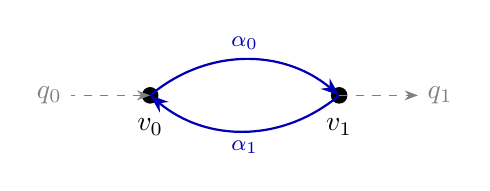
\begin{tikzpicture}[>=Stealth, scale=1.0]
  \fill (-1.2, 0) circle (3pt) node[below=5pt] {$v_0$};
  \fill ( 1.2, 0) circle (3pt) node[below=5pt] {$v_1$};
  \draw[->, thick, blue!70!black, bend left=40] (-1.2,0) to
    node[above, font=\footnotesize] {$\alpha_0$} (1.2,0);
  \draw[->, thick, blue!70!black, bend left=40] (1.2,0) to
    node[below, font=\footnotesize] {$\alpha_1$} (-1.2,0);
  \draw[<-, thin, dashed, gray] (-1.2,0) -- (-2.2,0) node[left] {$q_0$};
  \draw[->, thin, dashed, gray] (1.2,0) -- (2.2,0) node[right] {$q_1$};
\end{tikzpicture}
\end{center}

\subsection{Step 5: Kirchhoff Polynomial}

The reduced symbolic Laplacian $L_{RS} = E_{[\Gamma]}^T D_\alpha E_{[\Gamma]}$
for this graph (1 internal vertex after deleting $v_\infty$) has cofactor:
\begin{equation}
K(\alpha) = \alpha_0 + \alpha_1
\end{equation}

Each monomial is a spanning tree: $\{e_0\}$ with weight $\alpha_0$
and $\{e_1\}$ with weight $\alpha_1$.

\noindent\textbf{Code:}
\begin{verbatim}
G = FeynmanGraph(2, [(0,1,False), (1,0,False),
                      (2,0,True), (1,2,True)])
K = G.kirchhoff_polynomial()   # alpha0 + alpha1
trees = G.spanning_trees_from_kirchhoff()  # [[0], [1]]
\end{verbatim}

\subsection{Step 6: Symanzik Polynomial $\Psi$}

The first Symanzik polynomial is the complement of $K$ --- for each
spanning tree, take the product of edges \emph{not} in the tree:

\begin{center}
\begin{tabular}{llll}
\toprule
Tree $T$ & Edges in $T$ & Complement $\bar{T}$ & Monomial $\prod_{e \notin T} \alpha_e$ \\
\midrule
$T_0$ & $\{e_0\}$ & $\{e_1\}$ & $\alpha_1$ \\
$T_1$ & $\{e_1\}$ & $\{e_0\}$ & $\alpha_0$ \\
\bottomrule
\end{tabular}
\end{center}

\begin{equation}
\boxed{\Psi = \alpha_0 + \alpha_1}
\qquad\text{(homogeneous degree $L = 1$\; \checkmark)}
\end{equation}

\noindent\textbf{Code:}
\begin{verbatim}
sym = SymanzikPolynomials(G)
Psi = sym.Psi   # alpha0 + alpha1
sym.verify_homogeneity()  # {'Psi_homogeneous_degree_L': True}
\end{verbatim}

\subsection{Step 7: Degree of Divergence}

\begin{equation}
\sigma_d(G) = |E_{\mathrm{int}}| - \frac{d}{2}\,L = 2 - \frac{d}{2}
\end{equation}

At $d = d_c = 2$: $\sigma_2 = 1$ (logarithmic divergence $\to$ $1/\epsilon$ pole).

\subsection{Summary: The Full Chain}

\begin{tcolorbox}[colback=blue!3, colframe=deepblue, arc=4pt, breakable]
\small
\begin{center}
$\underset{\text{stoichiometry}}{S = (2,\,0)}$
$\;\xrightarrow{\text{Eq.\,(1)}}\;$
$\underset{\text{generator}}{Q = -\lambda(z^2{+}2z)\partial_z^2}$
$\;\xrightarrow{\text{expand}}\;$
$\underset{\text{vertices}}{\tilde\phi^2\phi^2,\; \tilde\phi^1\phi^2}$
$\;\xrightarrow{\text{pair}}\;$
$\underset{\text{loop diagram}}{%
\raisebox{-4pt}{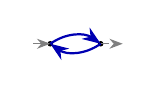
\begin{tikzpicture}[>=Stealth, scale=0.4]
\fill (-0.8,0) circle (2.5pt);
\fill (0.8,0) circle (2.5pt);
\draw[->, thick, blue!70!black, bend left=35] (-0.8,0) to (0.8,0);
\draw[->, thick, blue!70!black, bend left=35] (0.8,0) to (-0.8,0);
\draw[<-, thin, dashed, gray] (-0.8,0) -- (-1.5,0);
\draw[->, thin, dashed, gray] (0.8,0) -- (1.5,0);
\end{tikzpicture}}}$
$\;\xrightarrow{K}\;$
$\underset{\text{Kirchhoff}}{\alpha_0 {+} \alpha_1}$
$\;\xrightarrow{\text{compl.}}\;$
$\underset{\Psi}{\alpha_0 {+} \alpha_1}$
\end{center}
\smallskip
Every step is automated by \texttt{rdft}. Input: one line
(\texttt{ReactionNetwork.pair\_annihilation()}).
Output: the graph polynomials of every 1PI diagram at the desired loop order.
\end{tcolorbox}

\subsection{Automated Generation for Any Process}

The same chain runs for any CRN. For the Gribov process:

\begin{verbatim}
net = ReactionNetwork.gribov()
L = Liouvillian(net)
# Vertices: {(2,2): -chi, (2,1): beta, (1,2): -chi, (1,1): beta-eps}
exp = FeynmanExpansion(net, max_loops=1)
diagrams = exp.expand()
# diagrams[1] = list of all one-loop 1PI graphs with symmetry factors
for diag in diagrams[1]:
    G = diag['graph']
    sym = SymanzikPolynomials(G)
    print(f'Psi = {sym.Psi}, s(G) = {diag["symmetry_factor"]}')
\end{verbatim}

\subsection{Step 1: Extract Amputated vertexs from the Liouvillian}

Each monomial $\tilde\phi^m\phi^n$ in the Liouvillian $\mathcal{Q}$ with
$m+n \geq 3$ defines an \textbf{amputated vertex} --- a single vertex with $m$
outgoing half-edges ($\tilde\phi$ type) and $n$ incoming half-edges
($\phi$ type). For the Gribov process:

\begin{figure}[H]
\centering
% BRW Amputated vertexs — thesis Figure 3.3 style (auto-generated by rdft)
% Black solid arrows: A-species (walkers)
% Orange dashed arrows: B-species (tracers)
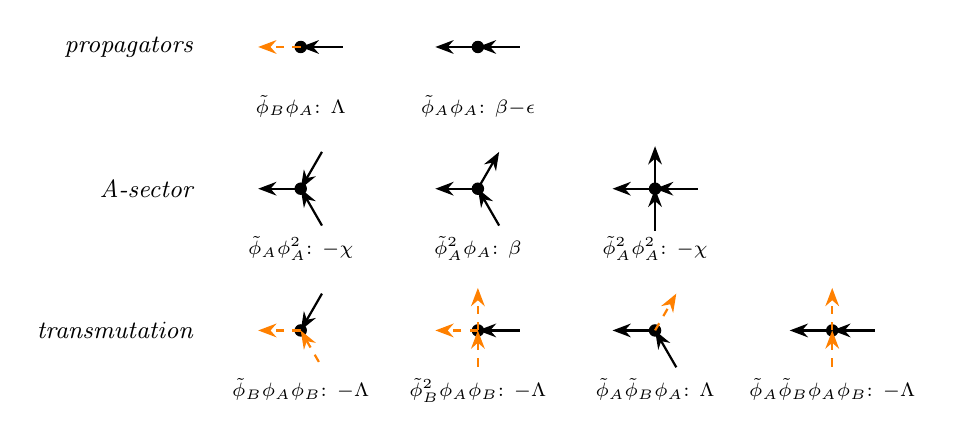
\begin{tikzpicture}[>=Stealth, scale=0.9]
  % --- Row 1: Propagators ---
  \fill (0.00,0.00) circle (2.5pt);
  \draw[->, thick, orange, dashed] (0.00,0.00) -- (-0.60,0.00);
  \draw[<-, thick] (0.00,0.00) -- (0.60,0.00);
  \node[below=10pt, font=\scriptsize] at (0.00,-0.15) {$\tilde{\phi}_B\phi_A$: $\Lambda$};
  \fill (2.50,0.00) circle (2.5pt);
  \draw[->, thick] (2.50,0.00) -- (1.90,0.00);
  \draw[<-, thick] (2.50,0.00) -- (3.10,0.00);
  \node[below=10pt, font=\scriptsize] at (2.50,-0.15) {$\tilde{\phi}_A\phi_A$: $\beta{-}\epsilon$};
  % --- Row 2: A-sector (black) ---
  \fill (0.00,-2.00) circle (2.5pt);
  \draw[->, thick] (0.00,-2.00) -- (-0.60,-2.00);
  \draw[<-, thick] (0.00,-2.00) -- (0.30,-1.48);
  \draw[<-, thick] (0.00,-2.00) -- (0.30,-2.52);
  \node[below=10pt, font=\scriptsize] at (0.00,-2.15) {$\tilde{\phi}_A\phi_A^2$: $-\chi$};
  \fill (2.50,-2.00) circle (2.5pt);
  \draw[->, thick] (2.50,-2.00) -- (1.90,-2.00);
  \draw[->, thick] (2.50,-2.00) -- (2.80,-1.48);
  \draw[<-, thick] (2.50,-2.00) -- (2.80,-2.52);
  \node[below=10pt, font=\scriptsize] at (2.50,-2.15) {$\tilde{\phi}_A^2\phi_A$: $\beta$};
  \fill (5.00,-2.00) circle (2.5pt);
  \draw[->, thick] (5.00,-2.00) -- (4.40,-2.00);
  \draw[->, thick] (5.00,-2.00) -- (5.00,-1.40);
  \draw[<-, thick] (5.00,-2.00) -- (5.60,-2.00);
  \draw[<-, thick] (5.00,-2.00) -- (5.00,-2.60);
  \node[below=10pt, font=\scriptsize] at (5.00,-2.15) {$\tilde{\phi}_A^2\phi_A^2$: $-\chi$};
  % --- Row 3: Transmutation (orange B-legs) ---
  \fill (0.00,-4.00) circle (2.5pt);
  \draw[->, thick, orange, dashed] (0.00,-4.00) -- (-0.60,-4.00);
  \draw[<-, thick] (0.00,-4.00) -- (0.30,-3.48);
  \draw[<-, thick, orange, dashed] (0.00,-4.00) -- (0.30,-4.52);
  \node[below=10pt, font=\scriptsize] at (0.00,-4.15) {$\tilde{\phi}_B\phi_A\phi_B$: $-\Lambda$};
  \fill (2.50,-4.00) circle (2.5pt);
  \draw[->, thick, orange, dashed] (2.50,-4.00) -- (1.90,-4.00);
  \draw[->, thick, orange, dashed] (2.50,-4.00) -- (2.50,-3.40);
  \draw[<-, thick] (2.50,-4.00) -- (3.10,-4.00);
  \draw[<-, thick, orange, dashed] (2.50,-4.00) -- (2.50,-4.60);
  \node[below=10pt, font=\scriptsize] at (2.50,-4.15) {$\tilde{\phi}_B^2\phi_A\phi_B$: $-\Lambda$};
  \fill (5.00,-4.00) circle (2.5pt);
  \draw[->, thick] (5.00,-4.00) -- (4.40,-4.00);
  \draw[->, thick, orange, dashed] (5.00,-4.00) -- (5.30,-3.48);
  \draw[<-, thick] (5.00,-4.00) -- (5.30,-4.52);
  \node[below=10pt, font=\scriptsize] at (5.00,-4.15) {$\tilde{\phi}_A\tilde{\phi}_B\phi_A$: $\Lambda$};
  \fill (7.50,-4.00) circle (2.5pt);
  \draw[->, thick] (7.50,-4.00) -- (6.90,-4.00);
  \draw[->, thick, orange, dashed] (7.50,-4.00) -- (7.50,-3.40);
  \draw[<-, thick] (7.50,-4.00) -- (8.10,-4.00);
  \draw[<-, thick, orange, dashed] (7.50,-4.00) -- (7.50,-4.60);
  \node[below=10pt, font=\scriptsize] at (7.50,-4.15) {$\tilde{\phi}_A\tilde{\phi}_B\phi_A\phi_B$: $-\Lambda$};
  % Row labels
  \node[left=15pt, font=\small\itshape] at (-0.8, 0) {propagators};
  \node[left=15pt, font=\small\itshape] at (-0.8, -2.0) {A-sector};
  \node[left=15pt, font=\small\itshape] at (-0.8, -4.0) {transmutation};
\end{tikzpicture}
\caption{Amputated vertices of the BRW, generated automatically
by \texttt{brw\_all\_vertices(max\_legs=4)}. Compare thesis Figure~3.3.
\textbf{Black solid arrows}: A-species (active walkers).
\textbf{Orange dashed arrows}: B-species (immobile tracers).
Row~1: propagator corrections.
Row~2: A-sector interactions (branching~$\beta$, coagulation~$\chi$).
Row~3: transmutation vertices from the carrying capacity trick
(thesis Eq.~3.21), coupling~$\Lambda$.
The dimensional filter \texttt{max\_legs=4} at $d_c = 4$ selects exactly
these 9 vertices from the 10 generated; one 5-leg vertex is irrelevant.}
\label{fig:corollas}
\end{figure}

\subsection{Step 2: Wick Contractions}

A \textbf{Wick contraction} pairs outgoing half-edges with incoming
half-edges to form internal propagators. Given a multiset of amputated vertices,
the algorithm:

\begin{enumerate}[leftmargin=2em]
\item Chooses $n$ interaction vertices ($m+n \geq 3$) from the vertex set.
\item Determines the required number of internal edges:
$E_{\mathrm{int}} = n + L - 1$ from the Betti number $L$.
\item Enumerates all partial matchings of $E_{\mathrm{int}}$ outgoing
half-edges with $E_{\mathrm{int}}$ incoming half-edges (partial permutations).
\item Builds a \texttt{FeynmanGraph} from each matching: paired half-edges
become internal edges; unpaired half-edges become external legs connected
to $v_\infty$.
\item Filters: keeps only \textbf{connected}, \textbf{1PI} (bridgeless) graphs
with the correct Betti number $L$.
\item Classifies by \textbf{graph isomorphism} (exact, via NetworkX) to
remove duplicates. The \textbf{symmetry factor} $s(G) = N_{\mathrm{total}} / N_{\mathrm{in\,class}}$.
\end{enumerate}

\subsection{Step 3: One-Loop Diagrams}

From the 9 amputated vertices, the code enumerates all possible vertex pairs
that can form one-loop ($L=1$) 1PI diagrams. There are 28 such pairs: 6
A-only and 22 mixed A/B. However, only the \textbf{A-sector} diagrams
contribute to the RG flow, because the B-species (immobile tracers) does
not diffuse and its propagator does not renormalise~\cite{nekovar2016,bordeu2019}.
The transmutation vertices couple the A-sector to the B-observable at
tree level only.

Of the 6 A-sector pairs, the thesis~\cite{amarteifio2019} shows that at
\textbf{vanishing external momentum} ($\hat{k} = \hat\omega = 0$), the
relevant diagrams (Eqs.~3.23a--b) are \textbf{loop-isomorphic}: they
evaluate to the same integral. Therefore only \textbf{one integral} needs
to be computed (thesis Eq.~3.24). The canonical diagram is:

\begin{figure}[H]
\centering
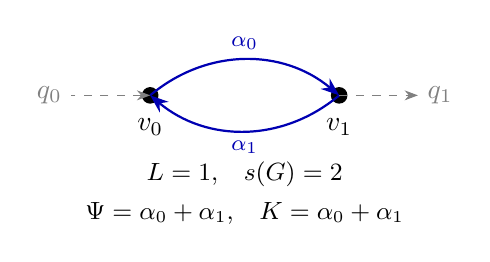
\begin{tikzpicture}[>=Stealth, scale=1.0]
  \fill (-1.2, 0) circle (3pt) node[below=5pt] {$v_0$};
  \fill ( 1.2, 0) circle (3pt) node[below=5pt] {$v_1$};
  \draw[->, thick, blue!70!black, bend left=40] (-1.2,0) to
    node[above, font=\footnotesize] {$\alpha_0$} (1.2,0);
  \draw[->, thick, blue!70!black, bend left=40] (1.2,0) to
    node[below, font=\footnotesize] {$\alpha_1$} (-1.2,0);
  \draw[<-, thin, dashed, gray] (-1.2,0) -- (-2.2,0) node[left] {$q_0$};
  \draw[->, thin, dashed, gray] (1.2,0) -- (2.2,0) node[right] {$q_1$};
  \node at (0,-1.0) {\small $L=1$,\quad $s(G) = 2$};
  \node at (0,-1.5) {\small $\Psi = \alpha_0 + \alpha_1$,\quad
    $K = \alpha_0 + \alpha_1$};
\end{tikzpicture}
\caption{One-loop self-energy diagram, automatically generated. The
Kirchhoff polynomial $K = \alpha_0 + \alpha_1$ (two spanning trees, one
per edge). The Symanzik polynomial $\Psi = \alpha_0 + \alpha_1$ (complement).
Symmetry factor $s(G) = 2$ from the EGF exponential formula.
Compare thesis Eq.~(3.24).}
\label{fig:oneloop_app}
\end{figure}

The code produces this diagram automatically:
\begin{verbatim}
from rdft import ReactionNetwork, Liouvillian
from rdft.core.expansion import FeynmanExpansion

net = ReactionNetwork.gribov()
exp = FeynmanExpansion(net, max_loops=1)
diagrams = exp.expand()
# diagrams[1] contains all one-loop 1PI graphs
\end{verbatim}

\section{Worked Integral: Graph Polynomials to UV Pole}
\label{app:integral}

We trace the complete ``scenic route'' calculation for the BRW one-loop
self-energy (thesis Example~2.5.15, Eqs.~2.102--2.103), showing how
the graph polynomials produce the amplitude step by step.

\subsection{The graph and its polynomials}

The one-loop self-energy has two propagators of species~$A$ with
diffusion constant~$D_A$ and mass $m_A$:

\begin{center}
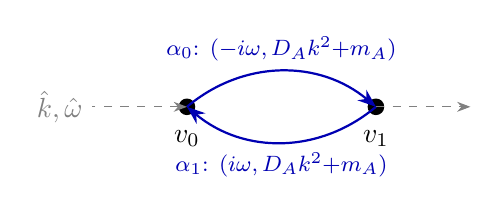
\begin{tikzpicture}[>=Stealth, scale=1.0]
  \fill (-1.2, 0) circle (3pt) node[below=5pt] {$v_0$};
  \fill ( 1.2, 0) circle (3pt) node[below=5pt] {$v_1$};
  \draw[->, thick, blue!70!black, bend left=40] (-1.2,0) to
    node[above, font=\footnotesize] {$\alpha_0$: $(-i\omega, D_Ak^2{+}m_A)$} (1.2,0);
  \draw[->, thick, blue!70!black, bend left=40] (1.2,0) to
    node[below, font=\footnotesize] {$\alpha_1$: $(i\omega, D_Ak^2{+}m_A)$} (-1.2,0);
  \draw[<-, thin, dashed, gray] (-1.2,0) -- (-2.4,0) node[left] {$\hat{k},\hat\omega$};
  \draw[->, thin, dashed, gray] (1.2,0) -- (2.4,0);
\end{tikzpicture}
\end{center}

From the incidence matrix (computed by \texttt{rdft}):
\begin{align}
\Psi &= \alpha_0 + \alpha_1 \qquad\text{(2 spanning trees, Kirchhoff complement)}
\label{eq:psi_example}\\
\Psi' &= D_A\alpha_0 + D_A\alpha_1 \qquad\text{(scaled by diffusion constants)}
\label{eq:psi_prime}\\
\frac{\Phi'}{\Psi'}\bigg|_{\hat k,\hat\omega=0}
&= \alpha_0(m_A - i\omega) + \alpha_1(m_A + i\omega) \qquad\text{(thesis Eq.~2.102)}
\label{eq:phi_prime}
\end{align}

\subsection{$\omega$-integration: the causal fingerprint}

The non-equilibrium $\omega$-integration applies $\delta(\Sigma_l)$ where
$\Sigma_l = \alpha_1 - \alpha_0$ is the circuit constraint from the edge-basis
matrix~$E_f$. This is Kirchhoff's frequency law on the single loop:
the sum of frequencies around the circuit vanishes.

After applying the $\delta$-function, the contracted graph $G'$ has one
fewer edge. The degree of divergence of the contracted graph is:
\begin{equation}
\sigma_d(G') = |E'| - \tfrac{d}{2}\,L' = 1 - d/2
\end{equation}

\subsection{The parametric integral}

Using the general parametric form~\cite{bogner2010,panzer2015} (thesis Eq.~2.99)
with $n_e = 1$ for all edges and the Schwinger
representation~\cite{schwinger1951}:
\begin{equation}
\mathcal{I}(G) = \Omega_d \cdot \Gamma\bigl(-\sigma_d(G')\bigr)
\int \dd\alpha_2 \; \frac{1}{(\Psi')^{d/2}}
\left(\frac{\Psi'}{\Phi'}\right)^{\!\sigma_d(G')}
\bigg|_{\alpha_2=1}
\end{equation}

Substituting the polynomials \eqref{eq:psi_prime}--\eqref{eq:phi_prime}
and using the Cheng--Wu theorem~\cite{chengwu1987} ($\alpha_2 = 1$ normalisation):
\begin{align}
\mathcal{I}(G)
&= \frac{\Gamma(1-d/2)}{(2\pi)^{d/2}}
\int \dd\alpha_2 \; \frac{1}{(2\alpha_2 D_A)^{d/2}}
\,[\alpha_2 \cdot 2m_A]^{\sigma_d(G')}
\bigg|_{\alpha_2=1}
\label{eq:integral_sub}\\
&= \frac{\Gamma(1-d/2)}{(2\pi)^{d/2}} \cdot \frac{1}{(2D_A)^{d/2}}
\cdot (2m_A)^{2/d-1}
\label{eq:integral_eval}\\
&= \mathcal{A}_d \cdot \Gamma(1-d/2) \cdot [2m_A]^{2/d-1}
\label{eq:integral_result}
\end{align}

where $\mathcal{A}_d = (4\pi D_A)^{-d/2}$ is the angular factor.

\begin{tcolorbox}[colback=blue!3, colframe=deepblue, arc=4pt]
\small
\textbf{What happened}: the graph polynomials $\Psi, \Phi$ (read from the
incidence matrix) and the $\delta$-function (from the edge-basis matrix)
reduced the integral to a \emph{single Gamma function} --- no momentum
integral was evaluated directly. The topology of the graph is encoded
in $\Psi$ and $\Phi$; the \emph{dimension} $d$ enters only through the
exponents $d/2$ and $\sigma_d$.
\end{tcolorbox}

\subsection{$\varepsilon$-expansion and the UV pole}

At the BRW upper critical dimension $d_c = 4$, set $d = 4 - \varepsilon$:
\begin{equation}
\Gamma(1 - d/2) = \Gamma(\varepsilon/2 - 1)
= \frac{-\Gamma(\varepsilon/2)}{1 - \varepsilon/2}
\xrightarrow{\varepsilon\to 0} \frac{-2}{\varepsilon} + \mathcal{O}(1)
\end{equation}

Including the symmetry factor $\mathfrak{s}(G) = 2$ (thesis Eq.~3.25):
\begin{equation}
\mathcal{I}_\lambda = \lambda \cdot \frac{\mathcal{A}_d}{\mathfrak{s}(G)}
\cdot \Gamma(\varepsilon/2) \cdot [1/\tilde{M}]^{\varepsilon/2}
\label{eq:amplitude_brw}
\end{equation}

The pole part (minimal subtraction, thesis Eq.~3.28):
\begin{equation}
\mathfrak{P}\!\left(\mathcal{I}_\lambda\right)
= \mu^\varepsilon \lambda_R \cdot \frac{\mathcal{A}_d}{\mathfrak{s}(G)}
\cdot \frac{2}{\varepsilon}
\end{equation}

This gives the $Z$-factor and $\beta$-function (thesis Eq.~3.30--3.31):
\begin{equation}
\boxed{Z_\lambda = 1 + \frac{\lambda}{(2\pi D)^2\,\varepsilon}
\qquad\Longrightarrow\qquad
\beta(\lambda) = \varepsilon\lambda_R + B\lambda_R^2,
\quad \lambda_R^* = \varepsilon/B}
\end{equation}

\noindent\textbf{Code:}
\begin{verbatim}
from rdft.graphs.incidence import FeynmanGraph
from rdft.integrals.symanzik import SymanzikPolynomials
G = FeynmanGraph.one_loop_self_energy()
sym = SymanzikPolynomials(G)
# Psi = alpha0 + alpha1, K = alpha0 + alpha1
# sigma_d = 2 - d/2, trees = [[0], [1]]
\end{verbatim}

The entire chain --- from incidence matrix to UV pole --- is automated by
\texttt{rdft}. The graph polynomial $\Psi$ determines the integral; the
dimension $d$ enters only as an exponent; and the pole $1/\varepsilon$ at
$d_c = 4$ produces the $Z$-factor that feeds the RG flow.
This is the scenic route; the AC route (Section~\ref{sec:ac_recovers_brw})
arrives at the same exponent without evaluating the integral.

\subsection{Connection to AC}

The Lagrange inversion coefficient $[g^n]\,G$ counts these diagrams:
\begin{equation}
[g^n]\, G = \frac{1}{n}\,[G^{n-1}]\,\phi(G)^n
= \text{(number of diagrams at loop order $n$, weighted by couplings)}
\end{equation}

This is the bridge between the AC route and the diagram route:
\emph{the same number} $[g^n]G$ can be computed either by Lagrange
inversion (algebraic) or by explicit enumeration (combinatorial).
The singularity of the GF $G(g)$ encodes the asymptotic growth
of this count, which is the content of the transfer theorem.

%% ================================================================
\section{The Kirchhoff Polynomial as a Generating Function}
\label{app:kirchhoff}

The Kirchhoff polynomial $K(\alpha) = \det(L_{RS})$, where $L_{RS}$ is
the cofactor of the reduced symbolic Laplacian, is itself a generating
function in the AC sense.

\subsection{The Matrix-Tree Theorem}

\begin{theorem}[Kirchhoff 1847~\cite{kirchhoff1847}]
For a connected graph $G$ with $n$ vertices and edge weights $\alpha_e$:
\begin{equation}
K(\alpha) = \sum_{T \in \mathcal{T}(G)} \prod_{e \in T} \alpha_e
\end{equation}
where $\mathcal{T}(G)$ is the set of spanning trees of $G$.
\end{theorem}

Each monomial in $K$ corresponds to a spanning tree. The number of
spanning trees is $K(1, 1, \ldots, 1)$.

\textbf{Example.} For the sunset diagram ($V=2$, $E_{\mathrm{int}}=3$):
\begin{equation}
K = \alpha_0 + \alpha_1 + \alpha_2
\qquad \text{(3 spanning trees, one per edge)}
\end{equation}

The code computes this automatically:
\begin{verbatim}
from rdft.graphs.incidence import FeynmanGraph
G = FeynmanGraph.sunset()
K = G.kirchhoff_polynomial()  # alpha0 + alpha1 + alpha2
trees = G.spanning_trees_from_kirchhoff()  # [[0], [1], [2]]
\end{verbatim}

\subsection{Symanzik $\Psi$ as the Complement}

The first Symanzik polynomial is the \textbf{complement} of $K$:
\begin{equation}
\Psi = \sum_{T \in \mathcal{T}(G)} \prod_{e \notin T} \alpha_e
\end{equation}
Each monomial has degree $L$ (the loop number) --- it is the product
of Schwinger parameters on the edges \emph{not} in the spanning tree
(the ``co-tree'' edges that form loops).

$\Psi$ is a generating function for the loop structure of $G$:
it counts, for each spanning tree, which edges form loops when
added back.

\subsection{AC Interpretation}

Both $K$ and $\Psi$ are generating functions in the combinatorial sense:
\begin{itemize}[leftmargin=2em]
\item $K$ is the OGF of spanning trees, weighted by edge parameters
\item $\Psi$ is the OGF of co-trees (loop structures)
\item The Matrix-Tree theorem is a special case of the
\textbf{transfer matrix method} in AC~\cite{flajolet2009}
\item The determinantal formula $K = \det(L_{RS})$ is the
\textbf{permanent/determinant} duality that connects Wick contractions
to graph polynomials
\end{itemize}

This is the ``scenic route'' version of what the AC route computes
directly: the Lagrange singularity encodes the \emph{asymptotic}
behaviour of these counts, without enumerating them.

\end{document}
